% Chapter 2

\chapter{无人机系统}
\section{系统硬件模块}
\subsection{整体硬件框架}
无人机系统是在DJI 经纬Matrice 100 (M100)无人机基础上搭建的,系统的硬件由飞控、机载电脑、传感器和外设四部分组成。其中飞控为DJI NI飞控,主要用来实现对无人机的直接控制,包含核心处理器(执行无人机的底层飞行控制操作)、串行通讯接口(与机载电脑通讯)、CAN通讯接口(与GPS模块、电机集成电调模块等通讯)、RF通讯接口(与DJI Lightbridge图传模块通讯)、多路PWM信号输出(用于控制旋翼电机转速)等;机载电脑是DJI Manifold妙算,主要用来执行目标检测与定位任务,以及控制无人机的自主飞行,Manifold妙算包含Tegra K1核心处理器(执行复杂算法和任务)、CAN通讯接口(接收云台相机采集的视频数据)、串行通讯接口(与飞控通讯)、USB接口(用于连接蓝牙串口模块和鼠标、键盘等设备)等;传感器包括云台相机(用于目标检测)、GPS模块(测量无人机的位置)、姿态传感器(测量无人机的姿态)等;外设包括蓝牙串口模块(与无人车通讯)、遥控器(用于设置无人机控制模式以及手动控制无人机)等。图~\ref{fig:2-1}为无人机系统的实物图,图~\ref{fig:2-2}为系统的整体硬件框架。

\clearpage 	
\begin{figure}[htb]
	\centering
	\begin{minipage}[t]{\linewidth} % 如果一行放2个图,用0.5,如果3个图,用0.33
		\centering
		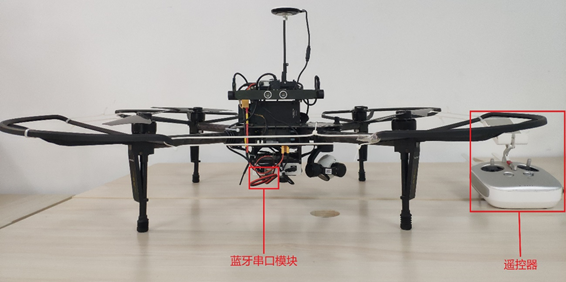
\includegraphics[width=\columnwidth]{figures/2-1a.png} 
		\subcaption{无人机系统实物图1} 
		\label{fig:2-1a}
	\end{minipage}
	\begin{minipage}[t]{\linewidth} 
		\centering
		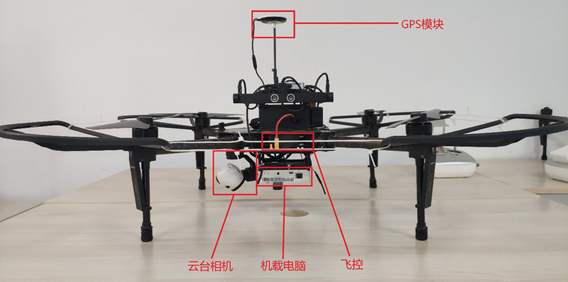
\includegraphics[width=\columnwidth]{figures/2-1b.png} 
		\subcaption{无人机系统实物图2} 
		\label{fig:2-1b} 
	\end{minipage}
	\caption{无人机系统实物图}
	\label{fig:2-1}
\end{figure}

\clearpage 	
\begin{figure}[htb]
	\centering
	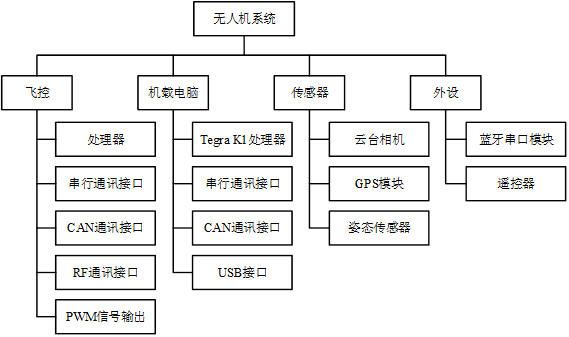
\includegraphics[width=\linewidth]{figures/2-2.png}
	\caption{无人机系统整体硬件框架}
	\label{fig:2-2}
\end{figure}

\subsection{飞控模块}
飞控,即飞行控制系统,是无人机的核心部件,其功能是接收GPS、IMU、气压计、磁力计等传感器数据,利用复杂算法计算得到飞行控制指令,并发送给执行机构,从而实现无人机的飞行、悬停、姿态控制、导航等任务。

本设计采用DJI M100自带的 N1飞控,N1飞控具有板载的IMU、气压计、磁力计等传感器,可用于测量无人机的高度和姿态。同时DJI N1飞控还搭载丰富的硬件接口,包含CAN通讯接口,用于与电调模块通讯,以及接收GPS数据;串行通讯接口,用于与机载电脑通讯;RF通讯接口,用于与DJI遥控器自带的Lightbridge图传模块通讯,传输云台相机拍摄的图像;Micro USB接口,用于PC端的飞行器仿真与飞控调参;PWM信号输出接口,用于控制旋翼电机转速。

\subsection{机载电脑}
机载电脑采用DJI推出的 Manifold妙算, 该机载电脑外型小巧,具有USB、Ethernet、HDMI、UART等多种接口,可连接鼠标、键盘、显示屏等扩展设备。

本设计中Manifold妙算主要用于控制无人机自主飞行,同时利用云台相机拍摄的图像进行目标的检测和定位,并通过蓝牙串口模块把目标的经纬度坐标数据发送给无人车。图~\ref{fig:2-3}为机载电脑Manifold妙算的外观和主要接口图。

\begin{figure}[htb]
	\begin{minipage}[t]{\linewidth}
		\centering
		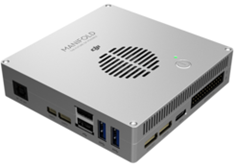
\includegraphics[width=0.5\columnwidth]{figures/2-3a.png} 
		\subcaption{Manifold妙算外观} 
		\label{fig:2-3a} 
	\end{minipage}
	\begin{minipage}[t]{\linewidth} 
		\centering
		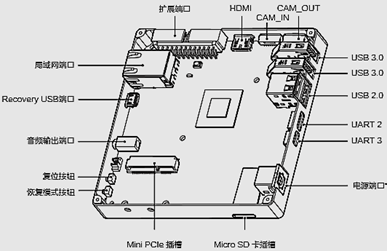
\includegraphics[width=0.8\columnwidth]{figures/2-3b.png} 
		\subcaption{Manifold妙算主要接口} 
		\label{fig:2-3b} 
	\end{minipage}
	\caption{机载电脑Manifold妙算\upcite{r35}}
	\label{fig:2-3}
\end{figure}

\subsection{云台相机}
云台相机采用DJI ZENMUSE X3一体化云台相机,该云台相机配置9组9片镜头,含2片非球面透镜,支持最高4K视频录制和1200万像素静态照片拍摄。三轴云台系统可实现360度无死角拍摄,云台可控转动范围,俯仰角为:+30°至-90°,翻滚角为:-90°至+60°,偏航角为:±320°。

该云台相机利用CAN总线传输视频信号,可以接入到N1飞控,再利用图传将视频信号传输到遥控器端,并利用手机等移动设备显示。也可以接入到机载电脑Manifold妙算,用于进行目标检测等操作。本系统中,首先将云台相机采集的视频信号通过CAN\_IN接口传输给Manifold妙算,Manifold妙算再通过CAN\_OUT接口传输给N1飞控,然后通过图传发送给遥控器,并通过手机显示。

图~\ref{fig:2-4}为DJI ZENMUSE X3云台相机的外观图。

\begin{figure}[htb]
	\centering
	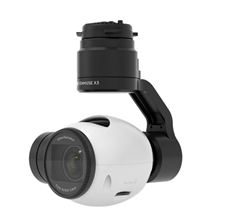
\includegraphics[width=0.4\linewidth]{figures/2-4.png}
	\caption{DJI ZENMUSE X3云台相机}
	\label{fig:2-4}
\end{figure}

\subsection{GPS模块}
GPS模块采用DJI M100无人机配套的GPS模块,定位精度可以达到米级。GPS模块通过CAN通讯接口连接到N1飞控,GPS信息将用于无人机的定位和导航,以及目标经纬度坐标的计算。图~\ref{fig:2-5}为GPS模块的外观图。

\begin{figure}[htb]
	\centering
	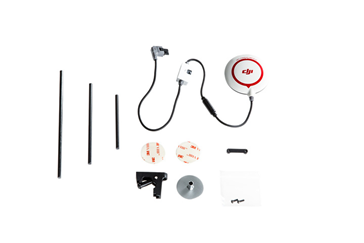
\includegraphics[width=0.6\linewidth]{figures/2-5.png}
	\caption{GPS模块}
	\label{fig:2-5}
\end{figure}

\subsection{姿态传感器}
姿态传感器采用N1飞控搭载的IMU+磁力计组合,通过IMU可以获得无人机的3轴加速度和3轴角速度,通过磁力计可以获得无人机所在位置的3轴磁感应强度,将加速度和磁感应强度进行融合可以求解出无人机的3轴姿态角(翻滚角$roll$、俯仰角$pitch$、偏航角$yaw$)。同时IMU数据也可以与GPS数据融合,用于提高无人机定位精度。本系统需要使用偏航角$yaw$进行无人机机体坐标系与局部坐标系的变换。

\subsection{蓝牙串口模块}
蓝牙串口模块选用的是HC-05主从一体蓝牙串口模块,这是一款低成本的蓝牙串口模块,兼容各种主流的串口波特率,可以直接与微控制器的UART接口相连,也可以结合USB转TTL芯片与PC或机载电脑相连。

本设计中无人机和无人车的机载电脑均搭载了蓝牙串口模块,一端作为主机,另一端作为从机,可以非常简便地实现无人机与无人车之间的无线数据传输。本设计中蓝牙串口模块用于传输目标的经纬度坐标数据。图~\ref{fig:2-6}为蓝牙串口模块的实物图。

\begin{figure}[htb]
	\centering
	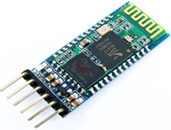
\includegraphics[width=0.4\linewidth]{figures/2-6.png}
	\caption{HC-05蓝牙串口模块}
	\label{fig:2-6}
\end{figure}

\subsection{遥控器}
遥控器使用DJI M100配套的DJI C1遥控器,该遥控器工作于2.4GHz频段,具有长达5千米的通信距离,并且集成了Lightbridge图传,可以直接输出航拍图像到手机等移动设备。

该遥控器可用于手动控制无人机,包括水平、垂直飞行以及旋转等操作,同时整合了相机操作以及云台操作的功能按键,以便用户在飞行时更轻松自如地航拍。当飞行模式切换到F挡时,允许利用机载电脑Manifold妙算控制无人机自主飞行。图~\ref{fig:2-7}为该遥控器的实物图。

\clearpage
\begin{figure}[htb]
	\centering
	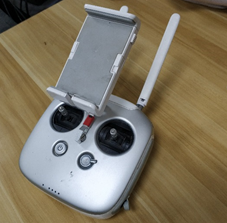
\includegraphics[width=0.4\linewidth]{figures/2-7.png}
	\caption{DJI C1遥控器}
	\label{fig:2-7}
\end{figure}

\section{目标检测算法}
\subsection{基准标记}
基准标记是一种用于快速检测的人工视觉特征图案,通常携带独一无二的编码信息用于区分不同的标记,并有相应的检测算法。基准标记类似于二维码,但降低了复杂度以满足实时性要求,其检测具有简单、快速、鲁棒、精确度高等特点。

基准标记最早在增强现实(augmented reality,简称AR)领域发展并流行起来,现已广泛用于机器人领域。基准标记具有目标检测识别、位姿估计、相机校准等功能。将基准标记贴附于目标物体表面,可以实现目标的快速检测和定位,同时利用基准标记独一无二的编码信息,还可以实现目标的识别和跟踪;利用基准标记作为路标,可用于机器人的定位和导航,以及作为SLAM等算法测试的ground truth。基准标记的检测一般分为3个步骤:标记的初检测;标记的精确定位;ID译码验证标记。

常用的基准标记有圆形基准标记和方形基准标记。圆形基准标记有CCC (concentric contrasting circle)\upcite{r10}、RuneTag\upcite{r11,r12}、CCTag\upcite{r13,r14}等,方形基准标记有ARTag\upcite{r15}、AprilTag\upcite{r16,r17}、ArUco\upcite{r18}等。多数基准标记都是黑白的,但也有少数彩色基准标记,例如Y. Cho等人改进的CCC标记\upcite{r19}、ChromaTag\upcite{r20}等。图~\ref{fig:2-8}展示了部分基准标记。

\clearpage
\begin{figure}[htb]
	\begin{minipage}[t]{0.33\linewidth}
		\centering
		
\includegraphics[width=\columnwidth]{figures/2-8a.png} 
		\subcaption{CCC\upcite{r10}} 
		\label{fig:2-8a} 
	\end{minipage}
	\begin{minipage}[t]{0.33\linewidth} 
		\centering
		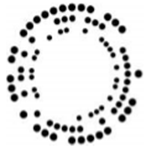
\includegraphics[width=\columnwidth]{figures/2-8b.png} 
		\subcaption{RuneTag\upcite{r11,r12}} 
		\label{fig:2-8b} 
	\end{minipage}
	\begin{minipage}[t]{0.33\linewidth} 
		\centering
		
\includegraphics[width=\columnwidth]{figures/2-8c.png} 
		\subcaption{CCTag\upcite{r13,r14}} 
		\label{fig:2-8c} 
	\end{minipage}
	\begin{minipage}[t]{0.33\linewidth}
		\centering
		
\includegraphics[width=\columnwidth]{figures/2-8d.png} 
		\subcaption{ARTag\upcite{r15}} 
		\label{fig:2-8d} 
	\end{minipage}
	\begin{minipage}[t]{0.33\linewidth} 
		\centering
		
\includegraphics[width=\columnwidth]{figures/2-8e.png} 
		\subcaption{AprilTag\upcite{r16,r17}} 
		\label{fig:2-8e} 
	\end{minipage}
	\begin{minipage}[t]{0.33\linewidth} 
		\centering
		
\includegraphics[width=\columnwidth]{figures/2-8f.png} 
		\subcaption{ArUco\upcite{r18}} 
		\label{fig:2-8f} 
	\end{minipage}
	\begin{minipage}[t]{0.33\linewidth} 
		\centering
		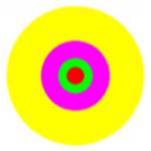
\includegraphics[width=\columnwidth]{figures/2-8g.png} 
		\subcaption{改进CCC\upcite{r19}} 
		\label{fig:2-8g} 
	\end{minipage}
	\begin{minipage}[t]{0.33\linewidth} 
		\centering
		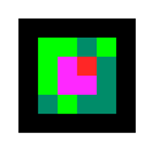
\includegraphics[width=\columnwidth]{figures/2-8h.png} 
		\subcaption{ChromaTag\upcite{r20}} 
		\label{fig:2-8h} 
	\end{minipage}
	\caption{部分基准标记}
	\label{fig:2-8}
\end{figure}

\subsection{AprilTag}
AprilTag是由Edwin Olson于2011年在ARTag基础上重新设计和实现的一种二进制方形基准标记\upcite{r16}。通过使用快速、鲁棒的线段检测算法,以及性能更好的数字编码算法,相较于之前的ARTag等基准标记,AprilTag具有更好的性能,包括更快的检测速度和更好的鲁棒性。图~\ref{fig:2-9}为三种不同型号的AprilTag。

\clearpage
\begin{figure}[htb]
	\begin{minipage}[t]{0.33\linewidth}
		\centering
		
\includegraphics[width=\columnwidth]{figures/2-9a.png} 
		\subcaption{4×4} 
		\label{fig:2-9a} 
	\end{minipage}
	\begin{minipage}[t]{0.33\linewidth} 
		\centering
		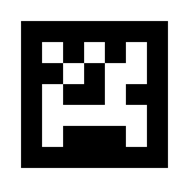
\includegraphics[width=\columnwidth]{figures/2-9b.png} 
		\subcaption{5×5} 
		\label{fig:2-9b} 
	\end{minipage}
	\begin{minipage}[t]{0.33\linewidth} 
		\centering
		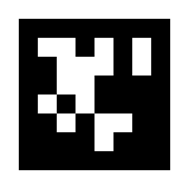
\includegraphics[width=\columnwidth]{figures/2-9c.png} 
		\subcaption{6×6} 
		\label{fig:2-9c} 
	\end{minipage}
	\caption{不同型号的AprilTag}
	\label{fig:2-9}
\end{figure}

AprilTag的检测算法分为以下4个步骤:

\begin{enumerate}[label=(\arabic*)] 
	\item 线段检测。首先计算每个像素的梯度方向和幅度,并通过聚类算法将梯度方向和幅度相似的像素点聚在一起。聚类算法类似于Felzenszwalb提出的基于图的图像分割算法\upcite{r21},首先创建一个图,每个节点代表一个像素,相邻节点之间添加一条边,权值为2个像素点的梯度方向之差,然后对这些边按权值进行升序排序,最后对于每条边,测试相连的2个节点所属的2个区域是否可以合并。其中,边的权值以定点数的形式存储,这样可以利用线性时间计数排序(linear-time counting sort)算法来加速边的排序,同时区域融合操作可以使用高效的并查集(union-find)算法来完成。另外基于梯度的聚类方法对噪声敏感,解决方案是对图像进行低通滤波。完成聚类操作后,再利用加权最小二乘算法对直线进行拟合,权重采用像素的梯度幅度。聚类算法是整个检测算法最慢的一个环节,可以采用对图像下采样的方法进行加速;
	\item 四边形检测。找到线段后,下一步就是四边形检测。作者采用了基于深度优先搜索(depth-first search,简称DFS)的方法,深度为4,每一次搜索添加一条边到四边形中。第一层时,遍历所有线段;第二至四层,寻找头部与上一层线段尾部“足够接近”并满足逆时针旋转顺序的线段。“足够接近”通过与阈值比较判断,作者将这个阈值设置得比较大,以得到较小的假阴性(false negative)比率,但也导致了较高的假阳性(false positive)比率,需要利用后续的译码来拒绝假阳性。另外作者使用了二维查找表进行四边形检测算法的加速。一旦四边形的四条边被找到,4个顶点可以通过计算线段的交点得到,由于线段是通过大量像素点拟合得到的,因此顶点的定位精度可以达到亚像素级别;
	\item 单应性和外参估计。通过直接线性变换(Direct Linear Transform,简称DLT)算法计算出单应性矩阵,然后利用单应性矩阵、相机内参和标记的物理尺寸计算出相机外参,详细的算法将在后面“PnP算法”一节介绍;
	\item ID译码。这一步的任务是读取标记中的二进制信息,首先通过单应性矩阵计算出每一个携带二进制信息的黑白网格对应的像素坐标,得到对应灰度值,然后通过灰度阈值判断其携带的二进制信息是0还是1,最后将二进制信息与码表匹配,验证是否为AprilTag基准标记,必要时可以采用纠错技术。为了增强对光照的鲁棒性,作者采用了随空间变化的灰度阈值,首先利用式~\eqref{eq2-1} 建立黑色像素模型和白色像素模型,然后利用黑白边界处两侧的灰度值通过最小二乘回归分别训练这两个模型,最后取两个模型的平均值作为灰度阈值。
\end{enumerate}

\begin{equation}\label{eq2-1}
	I(x, y) = A x + B x y + C y + D
\end{equation}

图~\ref{fig:2-10}为线段检测效果。

\begin{figure}[htb]
	\begin{minipage}[t]{0.33\linewidth}
		\centering
		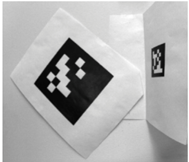
\includegraphics[width=\columnwidth]{figures/2-10a.png} 
		\subcaption{原图} 
		\label{fig:2-10a} 
	\end{minipage}
	\begin{minipage}[t]{0.33\linewidth} 
		\centering
		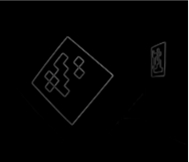
\includegraphics[width=\columnwidth]{figures/2-10b.png} 
		\subcaption{梯度幅度} 
		\label{fig:2-10b} 
	\end{minipage}
	\begin{minipage}[t]{0.33\linewidth} 
		\centering
		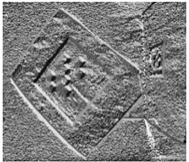
\includegraphics[width=\columnwidth]{figures/2-10c.png} 
		\subcaption{梯度方向可视化} 
		\label{fig:2-10c} 
	\end{minipage}
	\begin{minipage}[t]{0.33\linewidth}
		\centering
		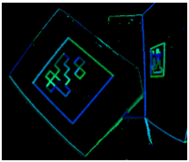
\includegraphics[width=\columnwidth]{figures/2-10d.png} 
		\subcaption{聚类结果} 
		\label{fig:2-10d} 
	\end{minipage}
	\begin{minipage}[t]{0.33\linewidth}
		\centering
		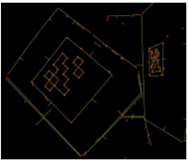
\includegraphics[width=\columnwidth]{figures/2-10e.png} 
		\subcaption{线段拟合结果} 
		\label{fig:2-10e} 
	\end{minipage}
	\caption{AprilTag线段检测效果\upcite{r16}}
	\label{fig:2-10}
\end{figure}

除了上述检测算法,作者还设计了编码算法,用于检错和纠错。对于编码算法,本文不做详细介绍。

2016年John Wang和Edwin Olson又对AprilTag进行了改进,提出了AprilTag2\upcite{r17}。相较于AprilTag,AprilTag2保留了编码算法,重新设计了检测算法,拥有了更快的检测速率和更高的准确率。

\subsection{ChromaTag}
之前的AprilTag等基准标记依赖于ID译码来拒绝假阳性,导致大量时间浪费在了最终会被当作假阳性拒绝的非标记区域的检测上,针对这一问题,Joseph DeGol等人在2017年基于AprilTag提出了一种彩色方形基准标记:ChromaTag\upcite{r20}。ChromaTag利用彩色信息快速拒绝假阳性,利用灰度信息实现精确定位,因此相较于之前的基准标记,具有显著的提速,同时达到了相似甚至更好的检测精度。

ChromaTag的图案设计如图~\ref{fig:2-11a}所示,最内层为红色(包括2种不同红色),往外是绿色(包括2种不同绿色),再往外是黑色,最外层是白色。检测时使用LAB色彩空间,图~\ref{fig:2-11a}所示标记图案的L、A、B通道分别如图~\ref{fig:2-11b}、~\ref{fig:2-11c}、~\ref{fig:2-11d}所示。在L通道下标记的黑白边界非常明显,在A通道下标记的红绿边界非常明显,在B通道下标记的2种红色和2种绿色差异明显。图~\ref{fig:2-12}为LAB色彩空间示意图。

\clearpage
\begin{figure}[htb]
	\begin{minipage}[t]{0.5\linewidth}
		\centering
		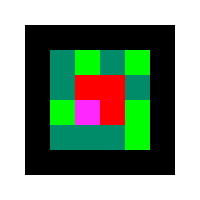
\includegraphics[width=0.7\columnwidth]{figures/2-11a.png} 
		\subcaption{原图} 
		\label{fig:2-11a} 
	\end{minipage}
	\begin{minipage}[t]{0.5\linewidth} 
		\centering
		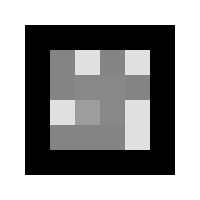
\includegraphics[width=0.7\columnwidth]{figures/2-11b.png} 
		\subcaption{L通道} 
		\label{fig:2-11b} 
	\end{minipage}
	\begin{minipage}[t]{0.5\linewidth} 
		\centering
		
\includegraphics[width=0.7\columnwidth]{figures/2-11c.png} 
		\subcaption{A通道} 
		\label{fig:2-11c} 
	\end{minipage}
	\begin{minipage}[t]{0.5\linewidth}
		\centering
		
\includegraphics[width=0.7\columnwidth]{figures/2-11d.png} 
		\subcaption{B通道} 
		\label{fig:2-11d} 
	\end{minipage}
	\caption{AprilTag的LAB图像}
	\label{fig:2-11}
\end{figure}

\begin{figure}[htb]
	\centering
	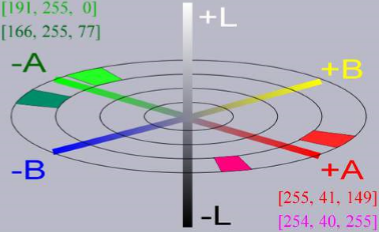
\includegraphics[width=0.5\linewidth]{figures/2-12.png}
	\caption{LAB色彩空间\upcite{r20}}
	\label{fig:2-12}
\end{figure}

根据ChromaTag的上述特性,可以利用A通道中红色和绿色的巨大差异进行标记的初步检测,利用L通道中黑白边界的高分辨率实现标记的精确定位,利用B通道中红色和绿色区域内部的差异进行ID编码和译码。ChromaTag可以直接由AprilTag生成,图~\ref{fig:2-13}显示了生成过程,最内层的4个黑白网格分别用2种不同红色代替,外层的12个黑白网格分别用2种不同绿色代替,即可得到ChromaTag。ChromaTag的编码与AprilTag相同。

\begin{figure}[htb]
	\centering
	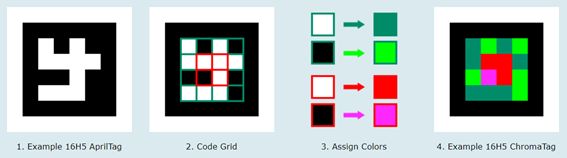
\includegraphics[width=\linewidth]{figures/2-13.png}
	\caption{AprilTag生成ChromaTag过程}
	\label{fig:2-13}
\end{figure}

ChromaTag的检测算法分为4个步骤:

\begin{enumerate}[label=(\arabic*)] 
	\item 扫描。以一定步长遍历整张图像,同时在A通道中做横向差分并与阈值比较,确定标记的起始中心点,然后向上下左右4个方向扫描,利用A通道的红绿差异和边界阈值确定4个红绿边界点,同时利用检测到的边界点坐标的均值更新标记中心点坐标,重复这个过程直到标记中心点收敛或者该点检测失败。若中心点收敛,则继续向上下左右4个方向扫描,利用L通道确定4个黑绿边界点和 4个黑白边界点;
	\item 构建多边形。利用第一步获得的12个边界点,构建3个初始多边形,这一步的任务是扩展这3个初始多边形,使其尽可能与标记的3条边界匹配。在可以使多边形面积增大最多的方向上扫描,确定下一个边界点并加入多边形中作为多边形的顶点,并通过多边形面积和相应阈值判断多边形是否收敛,重复此过程直到多边形收敛或扫描失败;
	\item 拟合四边形。对多边形的边利用边长作为权值进行加权的K-means\upcite{r22} (K=4)聚类,最终得到四边形的4条边,4个顶点通过计算4条边的交点得到,再利用Shi-Tomasi角点检测算法\upcite{r23}实现4个顶点的精确定位;
	\item ID译码。利用黑白边界的4个顶点求解单应性矩阵,通过单应性矩阵计算出红色和绿色网格对应的像素坐标,得到对应的B通道值,然后分别利用红色和绿色网格的B通道阈值判断其携带的二进制信息是0还是1。红色网格的B通道阈值为所有红色网格的B通道值的最大值和最小值的均值,绿色网格阈值类似。最后将二进制信息与码表匹配,验证是否为ChromaTag基准标记。
\end{enumerate}

图~\ref{fig:2-14}为ChromaTag检测流程。

\begin{figure}[htb]
	\centering
	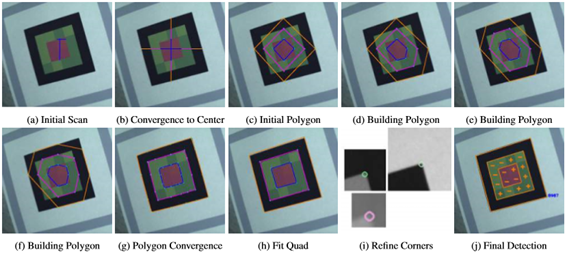
\includegraphics[width=\linewidth]{figures/2-14.png}
	\caption{ChromaTag检测流程\upcite{r20}}
	\label{fig:2-14}
\end{figure}

\subsection{ArUco}
对于之前的基准标记,其字典(基准标记的集合)的大小和标记间距(标记二进制码之间的汉明距离)都是固定的,因此存在两个问题,其一是在一些应用场景中所需标记数量可能超过字典大小,其二是如果所需标记数量很少,则使用一个更小的、具有更大标记间距的字典更为合适。同时之前的基准标记也不能很好地解决增强现实应用中的标记遮挡问题。

为了解决上述三个问题,S. Garrido-Jurado和R. Mun˜oz-Salinas等人在2014年提出了一种新的二进制方形基准标记:ArUco\upcite{r18}。首先,ArUco标记拥有可配置字典(字典大小和二进制码比特数可配置)生成算法,该算法遵循最大化标记间距和有效比特数的准则;其次,基于生成的字典,ArUco标记拥有自动检测和纠错算法;最后,ArUco标记采用多标记组合和基于颜色的遮挡区域计算方法,解决了标记的遮挡问题。

依靠可配置字典生成算法,ArUco标记具有很强的灵活性,可以根据需求生成对应大小的字典,同时保证最大化标记间距,既满足应用需求,又最大化检测的准确率。同时,ArUco标记的检测和纠错算法是一个通用框架,也可用于其他的基准标记,例如ARTag、AprilTag等。图~\ref{fig:2-15}为三种不同型号的ArUco标记。

\clearpage
\begin{figure}[htb]
	\begin{minipage}[t]{0.33\linewidth}
		\centering
		
\includegraphics[width=\columnwidth]{figures/2-15a.png} 
		\subcaption{4×4} 
		\label{fig:2-15a} 
	\end{minipage}
	\begin{minipage}[t]{0.33\linewidth} 
		\centering
		
\includegraphics[width=\columnwidth]{figures/2-15b.png} 
		\subcaption{5×5} 
		\label{fig:2-15b} 
	\end{minipage}
	\begin{minipage}[t]{0.33\linewidth} 
		\centering
		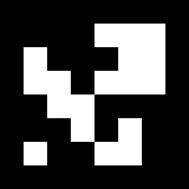
\includegraphics[width=\columnwidth]{figures/2-15c.png} 
		\subcaption{6×6} 
		\label{fig:2-15c} 
	\end{minipage}
	\caption{不同型号的ArUco标记}
	\label{fig:2-15}
\end{figure}

ArUco标记的检测过程分为以下4步:

\begin{enumerate}[label=(\arabic*)] 
	\item 图像分割。最初采用的是Canny边缘检测算法\upcite{r24},但不能满足实时检测的需求,后来选用了一种局部自适应阈值二值化的方法,该方法对于光照非常鲁棒;
	\item 轮廓提取和过滤。首先,在二值图中利用Suzuki和Abe的算法\upcite{r25}提取轮廓;接着利用Douglas和Peucker的算法\upcite{r26}对轮廓进行多边形近似,由于标记是方形的,因此可以过滤掉不能近似为四边形的轮廓;最后对于具有包含关系的轮廓,只保留最外面的一个;
	\item 标记二进制码提取。这一步是分析轮廓的内部区域来提取二进制码。首先计算单应性矩阵,并利用单应性矩阵去除相机的透视投影变换;接着利用大津法(Otsu)\upcite{r27}对图像做二值化;然后二值图被划分为均匀的网格,网格的每个元素根据内部多数像素的值被赋值为0或1;最后检测最外层网格元素是否全为0,判断标记的黑色边界是否存在,进行标记的第一步验证;
	\item 标记识别和纠错。一旦提取出候选标记的二进制码,就可以得到4种不同的ID (对应于4种可能的旋转),如果任意一种ID在字典中被找到,则认为候选标记有效,如果都没有找到,再使用纠错技术。
\end{enumerate}

ArUco标记的代码已经集成在opencv库中,同时AprilTag和ChromaTag的算法也是开源的,因此很方便进行测试,经过实验比较,本设计最终选用了性能最好的ArUco标记。

\section{目标定位算法}
\subsection{相机成像模型}
相机成像实际是将三维世界的点映射到二维像素平面的过程,可以使用简单的针孔模型\upcite{r28}来描述。针孔模型如图~\ref{fig:2-16}所示,其中$O-x-y-z$为相机坐标系,$z$轴指向相机前方,$x$轴向右,$y$轴向下,$O$为相机光心,也是针孔模型的针孔,$O'-x'-y'$为物理成像平面,相机的焦距为$f$。

\begin{figure}[htb]
	\centering
	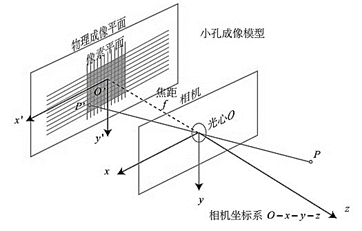
\includegraphics[width=0.6\linewidth]{figures/2-16.png}
	\caption{针孔相机模型\upcite{r28}}
	\label{fig:2-16}
\end{figure}

三维世界的点$P$经过小孔$O$投影到物理成像平面上的点$P'$。设在$O-x-y-z$坐标系下$P$的坐标为$\left[X,Y,Z\right]^T$,在$O'-x'-y'$坐标系下$P'$坐标$\left[X',Y'\right]^T$,根据三角形相似有:

\begin{equation}\label{eq2-2}
	\frac{Z}{f} = \frac{X}{X'} = \frac{Y}{Y'}
\end{equation}

整理得到:

\begin{equation}\label{eq2-3}
	\left\{ \begin{aligned}
		X' & = f \frac{X}{Z} \\
		Y' & = f \frac{Y}{Z} 
		\end{aligned}
	\right.
\end{equation}

成像之后还要进行采样和量化,才能得到像素图像。定义像素坐标系$o-u-v$在物理成像平面上,原点$o$位于图像的左上角,$u$轴向右与$x'$轴平行,$v$轴向下与$y'$轴平行,相对于$O'-x'-y'$坐标系,设原点平移了$\left[c_x,c_y\right]^T$,在$u$轴上缩放了$\alpha$倍,在v轴上缩放了$\beta$倍。同时设$P'$的像素坐标$\left[u,v\right]^T$,则有:

\begin{equation}\label{eq2-4}
	\left\{ \begin{aligned}
		u & = \alpha X' + c_x \\
		v & = \beta Y' +  c_y 
		\end{aligned}
	\right.
\end{equation}

代入式~\eqref{eq2-4},并令$f_x=\alpha f$,$f_y=\beta f$,得:

\begin{equation}\label{eq2-5}
	\left\{ \begin{aligned}
		u & = f_x \frac{X}{Z} + c_x \\
		v & = f_y \frac{Y}{Z} + c_y 
		\end{aligned}
	\right.
\end{equation}

写成矩阵形式,得:

\begin{equation}\label{eq2-6}
	Z \left[\begin{array}{c}u \\v \\ 1\end{array}\right] = \left[\begin{matrix}f_x & 0 & c_x \\ 0 & f_y & c_y \\ 0 & 0 & 1\end{matrix}\right] \triangleq K P
\end{equation}

式~\eqref{eq2-6}中,把中间的矩阵称为相机的内参数矩阵(Camera Intrinsics)$K$。一般认为相机的内参在是固定的,可以通过标定得到。

式~\eqref{eq2-6}中使用的是点$P$在相机坐标系下的坐标,可以由点$P$的世界坐标$P_w$通过相机的位姿变换得到,而相机的位姿可以用旋转矩阵$R$和平移向量$t$来描述,进而有:

\begin{equation}\label{eq2-7}
	Z P_{uv} = Z \left[\begin{array}{c}u \\ v \\ 1\end{array}\right] = K P = K \left(R P_w + t\right) = K T P_w
\end{equation}

其中$T=[R,t]$,注意这里隐含了非齐次坐标到齐次坐标的转换。

式~\eqref{eq2-7}描述了点$P$的世界坐标到像素坐标的投影关系。其中,相机的位姿$R$和$t$称为相机的外参数(Camera Extrinsics),相比于不变的内参,外参会随着相机的运动而变化。由于~\eqref{eq2-7}使用的是齐次坐标,因此可以把$Z$去掉,则有:

\begin{equation}\label{eq2-8}
	P_{uv} = K T P_w
\end{equation}

为了获得较好的成像效果,人们在相机的前方加入了透镜,这也导致了相机成像存在畸变,包括径向畸变和切向畸变。径向畸变可以用式~\eqref{eq2-9}纠正,切向畸变可以用式~\eqref{eq2-10}纠正。

\begin{equation}\label{eq2-9}
	\left\{ \begin{aligned}
		x_{corrected} & = x \left( 1 + k_1 r^2 + k_2 r^4 + k_3 r^6 \right) \\
		y_{corrected} & = y \left( 1 + k_1 r^2 + k_2 r^4 + k_3 r^6 \right)
		\end{aligned}
	\right.
\end{equation}

\begin{equation}\label{eq2-10}
	\left\{ \begin{aligned}
		x_{corrected} & = x + 2 p_1 x y + p_2 \left( r^2 + 2 x^2 \right) \\
		y_{corrected} & = y + 2 p_2 x y + p_1 \left( r^2 + 2 y^2 \right) 
		\end{aligned}
	\right.
\end{equation}

其中$\left[x,y\right]^T$为归一化坐标,$k$和$p$称为相机的畸变系数。相机的畸变模型\upcite{r28}可以用畸变系数来描述。

\subsection{PnP算法}
PnP (Perspective-n-Point)算法\upcite{r29}是通过$n$对3D与2D匹配点,利用最小化重投影误差来求解相机外参的算法,包括很多种求解方法,例如P3P\upcite{r30}、直接线性变换(DLT)\upcite{r31}、 EPnP (Efficient PnP)\upcite{r32}、UPnP\upcite{r33}等等。这里只介绍共面情况下基于单应性矩阵的求解方法。

根据前面介绍的相机成像模型,设三维世界坐标的点为$P_w=\left[X,Y,Z,1\right]^T$,对应二维像素坐标为$P_{uv}=\left[u,v,1\right]^T$,则有:

\begin{equation}\label{eq2-11}
	P_{uv} = K \left[ R, t \right] P_w
\end{equation}

将世界坐标系建立在基准标记平面上,并令基准标记平面为$Z=0$的平面,则有:

\begin{equation}\label{eq2-12}
	\left[\begin{array}{c} u \\ v \\ 1\end{array}\right] = K \left[ r_1 \quad r_2 \quad r_3 \quad t \right] \left[ \begin{array}{c} X \\ Y \\ 0 \\ 1\end{array}\right] = K \left[ r_1 \quad r_2 \quad t \right] \left[ \begin{array}{c} X \\ Y \\ 1\end{array}\right]
\end{equation}

我们把$K\left[r_1\quad r_2\quad t\right]$记作单应性矩阵$H$,则有:

\begin{equation}\label{eq2-13}
	\left[\begin{array}{c}u \\ v \\ 1 \end{array}\right] = H \left[\begin{array}{c} X \\ Y \\ 1 \end{array}\right]
\end{equation}

\begin{equation}\label{eq2-14}
	H = \left[ h_1 \quad h_2 \quad h_3\right] = \lambda K \left[ r_1 \quad r_2 \quad t \right]
\end{equation}

单应性矩阵$H$是一个$3 \times 3$的齐次矩阵,所以有8个未知数,而式~\eqref{eq2-13}包含2个方程,所以至少需要4对匹配点就可以计算出单应性矩阵$H$。而方形基准标记正好可以提供4个角点,并且通过基准标记的物理尺寸可以得到4个角点的世界坐标,因此可以很方便地计算出单应性矩阵$H$。

利用单应性矩阵可以计算出相机的内参和外参,这也是张正友相机标定算法\upcite{r34}的原理。而在已知相机内参的情况下,利用单应性矩阵计算相机外参则非常简单,由式~\eqref{eq2-14}可得:

\begin{equation}\label{eq2-15}
	\left\{ \begin{aligned}
		\lambda & = \frac{1}{\left\| K^{-1} h_1 \right\|} = \frac{1}{\left\| K^{-1} h_2 \right\|} \\
		r_1 & = \frac{1}{\lambda} K^{-1} h_1 \\
		r_2 & = \frac{1}{\lambda} K^{-1} h_2 \\
		r_3 & = r_1 \times r_2 \\
		t & = \lambda K^{-1} h_3
		\end{aligned}
	\right.
\end{equation}

式~\eqref{eq2-15}给出了外参的数值解,此外还可以通过迭代或优化的方式求解。

\subsection{GPS坐标计算}
利用PnP算法可以求出目标(基准标记)在相机坐标系下的坐标,此外还要利用相机坐标系与无人机机体坐标系的几何关系,以及无人机的偏航角和GPS坐标计算出目标的GPS坐标。

建立局部坐标系和机体坐标系如图~\ref{fig:2-17}所示。其中,$O-x-y-z$为局部坐标系,以无人机起点为原点,$x$轴指向北,$y$轴指向东,$z$轴向上,为左手系,便于与GPS坐标系进行坐标变化。$O'-x'-y'-z'$为机体坐标系,以无人机中心为原点,机身朝向为$x'$轴,$y'$轴向右,$z'$轴向上。无人机在飞行过程中可以认为保持水平,即$O'-x'-y'$平面与$O-x-y$平面平行,因此无人机的偏航角$yaw$就是$x'$轴与$x$轴的夹角。

\begin{figure}[htb]
	\centering
	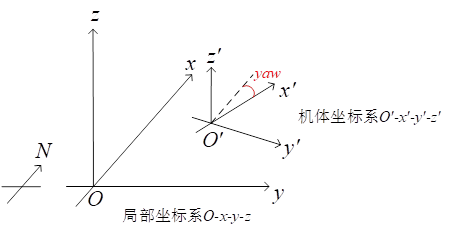
\includegraphics[width=0.6\linewidth]{figures/2-17.png}
	\caption{局部坐标系与机体坐标系}
	\label{fig:2-17}
\end{figure}

相机坐标系与机体坐标系的变换公式可以由云台相机与无人机中心的相对位置关系和云台的角度得到,本设计中保持云台相机竖直朝下,这样坐标变换会更加简单。设无人机在局部坐标系下坐标为$P_{lu}$,在GPS坐标系下坐标为$P_{gu}=\left[Lat0, Lon0, Alt0\right]^T$ (Lat0为维度,Lon0为经度,Alt0为高度,经纬度采用角度单位);目标在机体坐标系下坐标为$P_{bt}$,在局部坐标系下坐标为$P_{lt}$,在GPS坐标系下坐标为$P_{gt}=\left[Lat1,Lon1,Alt1\right]^T$,则有:

\begin{equation}\label{eq2-16}
	p_{lt} = \left[\begin{matrix} \cos(yaw) & -\sin(yaw) & 0 \\
	\sin(yaw) & \cos(yaw) & 0 \\ 0 & 0 & 1 \end{matrix}\right] P_{bt} + P_{lu} 
	= R P_{bt} + P_{lu} 
\end{equation}

在很小的范围内,将GPS坐标系近似为平面直角坐标系,并设地球半径为$r$,则有:

\begin{equation}\label{eq2-17}
	\left[\begin{array}{c} \Delta X \\ \Delta Y \\ \Delta Z \end{array}\right] = R P_{bt} 
\end{equation}

\begin{equation}\label{eq2-18}
	\left\{ \begin{aligned}
		\Delta Lat & \approx \frac{\Delta X}{r} \cdot \frac{180}{\pi} \\
		\Delta Lon & \approx \frac{\Delta Y}{r \cos(Lat0 \cdot \frac{\pi}{180})} \cdot \frac{180}{\pi} \\
		\Delta Lon & \approx \Delta Z
	\end{aligned}
	\right.
\end{equation}

\begin{equation}\label{eq2-19}
	P_{gt} = P_{gu} + \left[ \begin{array}{c} \Delta Lat \\ \Delta Lon \\ \Delta Alt \end{array}\right]
\end{equation}

利用式~\eqref{eq2-16}$\sim$~\eqref{eq2-19}即可求出目标的GPS坐标。

\section{无人机自主飞行}
无人机的自主飞行利用DJI 提供的Onboard SDK来实现。飞行任务分为以下3个步骤:

\begin{enumerate}[label=(\arabic*)] 
	\item 起飞。无人机垂直起飞到1.2m左右;
	\item 区域扫描。区域扫描采用设置航点任务的方式实现,航点坐标采用GPS坐标,可以利用式~\eqref{eq2-16}$\sim$~\eqref{eq2-19}求得,航点高度为3m。图~\ref{fig:2-18}为区域扫描示意图,无人机经过各个航点的顺序为$P_0 \to P_1 \to P_2 \to P_3 \to \cdots \to P_{N-2} \to P_{N-1} \to P_N \to P_0$,起点和终点均为$P_0$,起点的$P_0$用于让无人机上升到3m,终点的$P_0$用于让无人机降落到起飞点;
	\item 降落。完成扫描任务后降落到起飞点。
\end{enumerate}

\begin{figure}[htb]
	\centering
	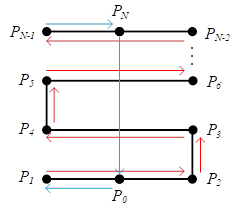
\includegraphics[width=0.4\linewidth]{figures/2-18.png}
	\caption{区域扫描示意图}
	\label{fig:2-18}
\end{figure}

\section{系统软件设计}
无人机系统的机载电脑Manifold妙算使用Ubuntu 14.04操作系统,并装有ROS (Robot Operating System,机器人操作系统),本项目利用opencv库实现了目标的检测与定位,利用ROS和DJI的Onboard SDK实现了无人机的自主飞行。图~\ref{fig:2-19}为无人机系统的软件流程图,系统首先设置云台角度使得云台相机竖直朝下,接着让无人机起飞,然后开始扫描待搜索区域,同时进行目标检测和定位,扫描结束后让无人机降落到初始位置,最后发送目标位置信息给无人车。

\begin{figure}[htb]
	\centering
	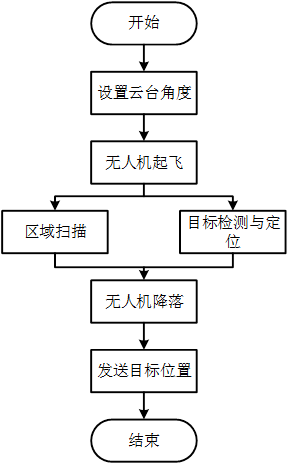
\includegraphics[width=0.4\linewidth]{figures/2-19.png}
	\caption{无人机系统软件流程图}
	\label{fig:2-19}
\end{figure}

\section{本章小结}
本章首先介绍了无人机系统的硬件框架和模块,接着利用基准标记作为搜索目标,介绍了AprilTag、ChromaTag和ArUco三种基准标记的检测算法,以及基于PnP算法的基准标记定位算法,然后简要描述了如何实现无人机的自主飞行,最后介绍了系统的软件设计。


